\documentclass[11pt, a4paper]{article}

% --- UNIVERSAL PREAMBLE ---
\usepackage[a4paper, top=2.5cm, bottom=2.5cm, left=2cm, right=2cm]{geometry}
\usepackage{amsmath}

% --- GRAPHICS PACKAGES ---
\usepackage{tikz}
\usetikzlibrary{positioning, arrows.meta, shapes.geometric, calc, decorations.pathreplacing}
\usepackage{xcolor} % Required for custom colors

% ==========================================
%   UNIVERSITY OF SOUTH CAROLINA COLORS
% ==========================================
% Primary Colors
\definecolor{UofSCGarnet}{RGB}{115, 0, 10}
\definecolor{UofSCBlack}{RGB}{0, 0, 0}
\definecolor{UofSCWhite}{RGB}{255, 255, 255}

% Neutral Colors
\definecolor{UofSC90Black}{RGB}{54, 54, 54}
\definecolor{UofSC70Black}{RGB}{92, 92, 92}
\definecolor{UofSC50Black}{RGB}{162, 162, 162}
\definecolor{UofSC30Black}{RGB}{199, 199, 199}
\definecolor{UofSC10Black}{RGB}{235, 235, 235}
\definecolor{UofSCWarmGrey}{RGB}{103, 97, 86}
\definecolor{UofSCSandstorm}{RGB}{255, 242, 227}

% Accent Colors
\definecolor{UofSCRose}{RGB}{204, 46, 64}
\definecolor{UofSCAtlantic}{RGB}{70, 106, 159}
\definecolor{UofSCCongaree}{RGB}{31, 65, 77}
\definecolor{UofSCHorseshoe}{RGB}{101, 120, 11}
\definecolor{UofSCGrass}{RGB}{206, 211, 24}
\definecolor{UofSCHoneycomb}{RGB}{164, 145, 55}

% Special Use Colors
\definecolor{UofSCDarkGarnet}{RGB}{87, 0, 8}
\definecolor{UofSCAzalea}{RGB}{132, 66, 71}

% ==========================================
%      CONFIGURATION & COLOR PALETTE
% ==========================================
% Main (I-frame / independent) elements
\colorlet{FrameFill}{UofSCSandstorm}      % Warm light background
\colorlet{FrameStroke}{UofSCGarnet}       % Garnet outline

\colorlet{EncoderFill}{UofSCWhite}        % White interior
\colorlet{EncoderStroke}{UofSCGarnet}     % Garnet outline

% Diff (D-frame) elements -- used only in second diagram
% Make D-frames blue and their encoders a teal/blue fill
\colorlet{DiffFrameFill}{UofSCAtlantic!30}    % Medium blue fill
\colorlet{DiffFrameStroke}{UofSCCongaree}  % Dark blue-green outline

\colorlet{DiffEncoderFill}{UofSCAtlantic!30}  % Teal/blue fill (not white)
\colorlet{DiffEncoderStroke}{UofSCCongaree}% Blue outline


% Network Bar Colors
\colorlet{NetworkFill}{UofSC10Black}      % Very light neutral background
\colorlet{NetworkStroke}{UofSC90Black}    % Dark neutral outline
\colorlet{NetworkText}{UofSCBlack}        % Black text

% Arrow Colors
\colorlet{ArrowColor}{UofSCGarnet}        % Garnet arrows

% ==========================================
%            TIKZ STYLES
% ==========================================
\tikzset{
    % Standard Frame (F1, F2...)
    sketchframe/.style={
        draw=FrameStroke,
        fill=FrameFill,
        trapezium,
        trapezium left angle=70,
        trapezium right angle=110,
        minimum width=1cm,
        minimum height=0.8cm,
        font=\small\itshape,
        thick
    },
    % Diff Frame (D / "Diff" frames)
    sketchframeDiff/.style={
        draw=DiffFrameStroke,
        fill=DiffFrameFill,
        trapezium,
        trapezium left angle=70,
        trapezium right angle=110,
        minimum width=1cm,
        minimum height=0.8cm,
        font=\small\itshape,
        thick
    },
    % Encoder Circle (enc)
    sketchenc/.style={
        draw=EncoderStroke,
        fill=EncoderFill,
        circle,
        minimum size=0.9cm,
        inner sep=1pt,
        font=\footnotesize,
        thick
    },
    % Diff Encoder Circle
    sketchencDiff/.style={
        draw=DiffEncoderStroke,
        fill=DiffEncoderFill,
        circle,
        minimum size=0.9cm,
        inner sep=1pt,
        font=\footnotesize,
        thick
    },
    % Network Bar (The long rectangle)
    network/.style={
        draw=NetworkStroke,
        fill=NetworkFill,
        text=NetworkText,
        rectangle,
        minimum height=1cm,
        align=center,
        font=\small\bfseries\sffamily,
        thick
    },
    % Standard Arrow Style
    stdarrow/.style={
        ->,
        >=Latex,
        thick,
        color=ArrowColor
    },
    % Dashed Arrow Style
    dasharrow/.style={
        ->,
        >=Latex,
        thick,
        dashed,
        color=ArrowColor
    }
}

\begin{document}

\begin{figure}[htbp]
\centering
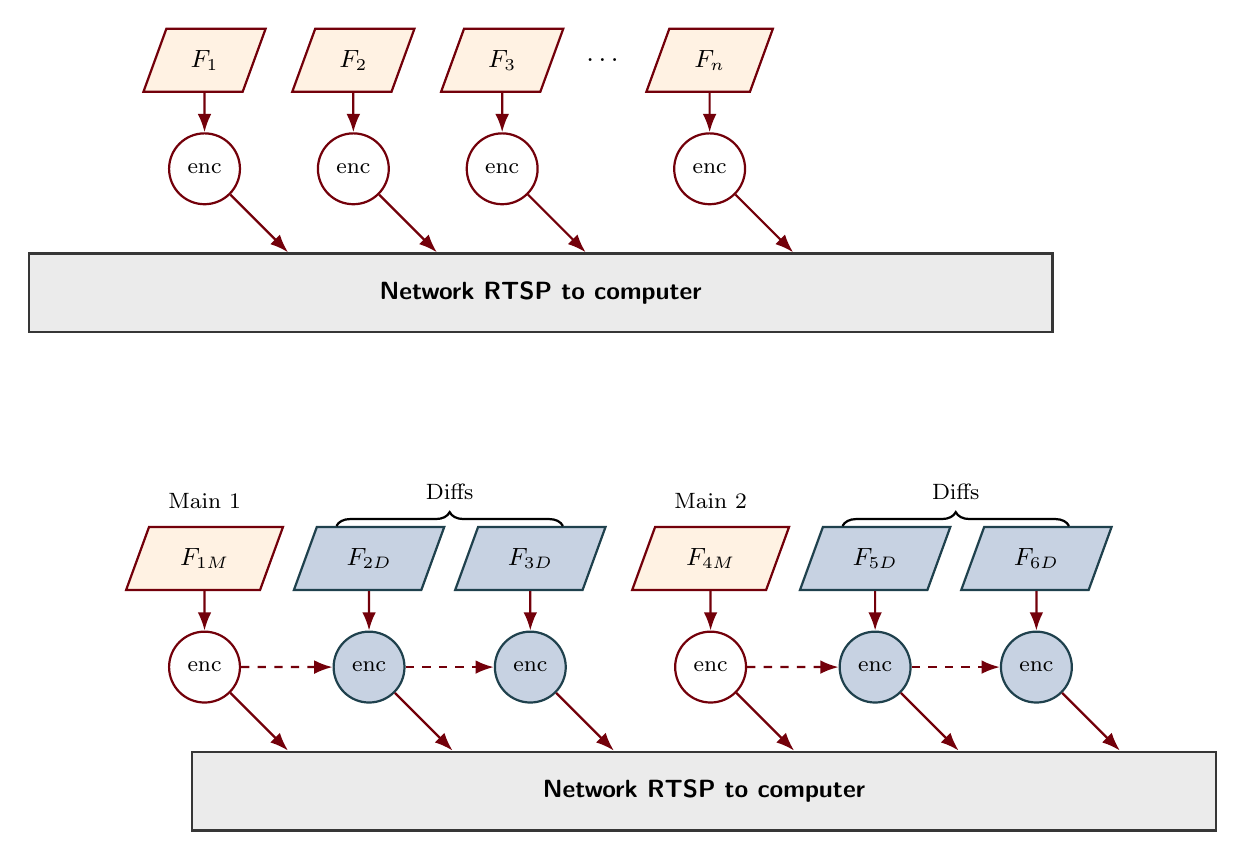
\begin{tikzpicture}[node distance=1.2cm]

    % ==========================================
    % TOP DIAGRAM: MJPEG / INDEPENDENT FRAMES
    % ==========================================
    
    % Frames
    \node[sketchframe] (mf1) at (0, 1) {$F_1$};
    \node[sketchframe, right=0.6cm of mf1] (mf2) {$F_2$};
    \node[sketchframe, right=0.6cm of mf2] (mf3) {$F_3$};
    \node[right=0.3cm of mf3] (mdots) {$\dots$};
    \node[sketchframe, right=0.3cm of mdots] (mfn) {$F_n$};
    
    % Encoders & Vertical Arrows
    \foreach \f/\e in {mf1/me1, mf2/me2, mf3/me3, mfn/men} {
        \node[sketchenc, below=0.5cm of \f] (\e) {enc};
        \draw[stdarrow] (\f) -- (\e);
        \draw[stdarrow] (\e) -- +(-45:1.5) coordinate (tip\e);
    }
    
    % Network Bar (Top)
    \path (tipme1) -- (tipmen) coordinate[midway] (mid1);
    \node[network, minimum width=13cm, anchor=north] (net1) at (mid1) {Network RTSP to computer};


    % ==========================================
    % BOTTOM DIAGRAM: H.264 / INTER-FRAME
    % ==========================================
    
    % Cycle 1 Nodes
    \node[sketchframe, below=5.5cm of mf1] (h1) {$F_{1M}$};
    \node[above=0.1cm of h1, font=\footnotesize] {Main 1};
    
    \node[sketchframeDiff, right=0.4cm of h1] (h2) {$F_{2D}$};
    \node[sketchframeDiff, right=0.4cm of h2] (h3) {$F_{3D}$};
    
    % Brace Cycle 1
    \draw[decoration={brace,amplitude=5pt}, decorate, thick] 
        (h2.north west) -- (h3.north east) 
        node [midway, above=6pt, font=\footnotesize] {Diffs};

    % Cycle 2 Nodes
    \node[sketchframe, right=0.6cm of h3] (h4) {$F_{4M}$};
    \node[above=0.1cm of h4, font=\footnotesize] {Main 2};
    
    \node[sketchframeDiff, right=0.4cm of h4] (h5) {$F_{5D}$};
    \node[sketchframeDiff, right=0.4cm of h5] (h6) {$F_{6D}$};
    
    % Brace Cycle 2
    \draw[decoration={brace,amplitude=5pt}, decorate, thick] 
        (h5.north west) -- (h6.north east) 
        node [midway, above=6pt, font=\footnotesize] {Diffs};
        
    % Encoders & Network Links (explicit to distinguish Main vs Diff)
    % h1 (Main)
    \node[sketchenc, below=0.5cm of h1] (he1) {enc};
    \draw[stdarrow] (h1) -- (he1);
    \draw[stdarrow] (he1) -- +(-45:1.5) coordinate (tiphe1);

    % h2 (Diff)
    \node[sketchencDiff, below=0.5cm of h2] (he2) {enc};
    \draw[stdarrow] (h2) -- (he2);
    \draw[stdarrow] (he2) -- +(-45:1.5) coordinate (tiphe2);

    % h3 (Diff)
    \node[sketchencDiff, below=0.5cm of h3] (he3) {enc};
    \draw[stdarrow] (h3) -- (he3);
    \draw[stdarrow] (he3) -- +(-45:1.5) coordinate (tiphe3);

    % h4 (Main)
    \node[sketchenc, below=0.5cm of h4] (he4) {enc};
    \draw[stdarrow] (h4) -- (he4);
    \draw[stdarrow] (he4) -- +(-45:1.5) coordinate (tiphe4);

    % h5 (Diff)
    \node[sketchencDiff, below=0.5cm of h5] (he5) {enc};
    \draw[stdarrow] (h5) -- (he5);
    \draw[stdarrow] (he5) -- +(-45:1.5) coordinate (tiphe5);

    % h6 (Diff)
    \node[sketchencDiff, below=0.5cm of h6] (he6) {enc};
    \draw[stdarrow] (h6) -- (he6);
    \draw[stdarrow] (he6) -- +(-45:1.5) coordinate (tiphe6);
    
    % Network Bar (Bottom)
    \path (tiphe1) -- (tiphe6) coordinate[midway] (mid2);
    \node[network, minimum width=13cm, anchor=north] (net2) at (mid2) {Network RTSP to computer};
    
    % Dependency Arrows (Horizontal Dashed)
    \draw[dasharrow] (he1) -- (he2);
    \draw[dasharrow] (he2) -- (he3);
    \draw[dasharrow] (he4) -- (he5);
    \draw[dasharrow] (he5) -- (he6);

\end{tikzpicture}
\end{figure}

\end{document}
